\documentclass[1p]{elsarticle_modified}
%\bibliographystyle{elsarticle-num}

%\usepackage[colorlinks]{hyperref}
%\usepackage{abbrmath_seonhwa} %\Abb, \Ascr, \Acal ,\Abf, \Afrak
\usepackage{amsfonts}
\usepackage{amssymb}
\usepackage{amsmath}
\usepackage{amsthm}
\usepackage{scalefnt}
\usepackage{amsbsy}
\usepackage{kotex}
\usepackage{caption}
\usepackage{subfig}
\usepackage{color}
\usepackage{graphicx}
\usepackage{xcolor} %% white, black, red, green, blue, cyan, magenta, yellow
\usepackage{float}
\usepackage{setspace}
\usepackage{hyperref}

\usepackage{tikz}
\usetikzlibrary{arrows}

\usepackage{multirow}
\usepackage{array} % fixed length table
\usepackage{hhline}

%%%%%%%%%%%%%%%%%%%%%
\makeatletter
\renewcommand*\env@matrix[1][\arraystretch]{%
	\edef\arraystretch{#1}%
	\hskip -\arraycolsep
	\let\@ifnextchar\new@ifnextchar
	\array{*\c@MaxMatrixCols c}}
\makeatother %https://tex.stackexchange.com/questions/14071/how-can-i-increase-the-line-spacing-in-a-matrix
%%%%%%%%%%%%%%%

\usepackage[normalem]{ulem}

\newcommand{\msout}[1]{\ifmmode\text{\sout{\ensuremath{#1}}}\else\sout{#1}\fi}
%SOURCE: \msout is \stkout macro in https://tex.stackexchange.com/questions/20609/strikeout-in-math-mode

\newcommand{\cancel}[1]{
	\ifmmode
	{\color{red}\msout{#1}}
	\else
	{\color{red}\sout{#1}}
	\fi
}

\newcommand{\add}[1]{
	{\color{blue}\uwave{#1}}
}

\newcommand{\replace}[2]{
	\ifmmode
	{\color{red}\msout{#1}}{\color{blue}\uwave{#2}}
	\else
	{\color{red}\sout{#1}}{\color{blue}\uwave{#2}}
	\fi
}

\newcommand{\Sol}{\mathcal{S}} %segment
\newcommand{\D}{D} %diagram
\newcommand{\A}{\mathcal{A}} %arc


%%%%%%%%%%%%%%%%%%%%%%%%%%%%%5 test

\def\sl{\operatorname{\textup{SL}}(2,\Cbb)}
\def\psl{\operatorname{\textup{PSL}}(2,\Cbb)}
\def\quan{\mkern 1mu \triangleright \mkern 1mu}

\theoremstyle{definition}
\newtheorem{thm}{Theorem}[section]
\newtheorem{prop}[thm]{Proposition}
\newtheorem{lem}[thm]{Lemma}
\newtheorem{ques}[thm]{Question}
\newtheorem{cor}[thm]{Corollary}
\newtheorem{defn}[thm]{Definition}
\newtheorem{exam}[thm]{Example}
\newtheorem{rmk}[thm]{Remark}
\newtheorem{alg}[thm]{Algorithm}

\newcommand{\I}{\sqrt{-1}}
\begin{document}

%\begin{frontmatter}
%
%\title{Boundary parabolic representations of knots up to 8 crossings}
%
%%% Group authors per affiliation:
%\author{Yunhi Cho} 
%\address{Department of Mathematics, University of Seoul, Seoul, Korea}
%\ead{yhcho@uos.ac.kr}
%
%
%\author{Seonhwa Kim} %\fnref{s_kim}}
%\address{Center for Geometry and Physics, Institute for Basic Science, Pohang, 37673, Korea}
%\ead{ryeona17@ibs.re.kr}
%
%\author{Hyuk Kim}
%\address{Department of Mathematical Sciences, Seoul National University, Seoul 08826, Korea}
%\ead{hyukkim@snu.ac.kr}
%
%\author{Seokbeom Yoon}
%\address{Department of Mathematical Sciences, Seoul National University, Seoul, 08826,  Korea}
%\ead{sbyoon15@snu.ac.kr}
%
%\begin{abstract}
%We find all boundary parabolic representation of knots up to 8 crossings.
%
%\end{abstract}
%\begin{keyword}
%    \MSC[2010] 57M25 
%\end{keyword}
%
%\end{frontmatter}

%\linenumbers
%\tableofcontents
%
\newcommand\colored[1]{\textcolor{white}{\rule[-0.35ex]{0.8em}{1.4ex}}\kern-0.8em\color{red} #1}%
%\newcommand\colored[1]{\textcolor{white}{ #1}\kern-2.17ex	\textcolor{white}{ #1}\kern-1.81ex	\textcolor{white}{ #1}\kern-2.15ex\color{red}#1	}

{\Large $\underline{12n_{0009}~(K12n_{0009})}$}

\setlength{\tabcolsep}{10pt}
\renewcommand{\arraystretch}{1.6}
\vspace{1cm}\begin{tabular}{m{100pt}>{\centering\arraybackslash}m{274pt}}
\multirow{5}{120pt}{
	\centering
	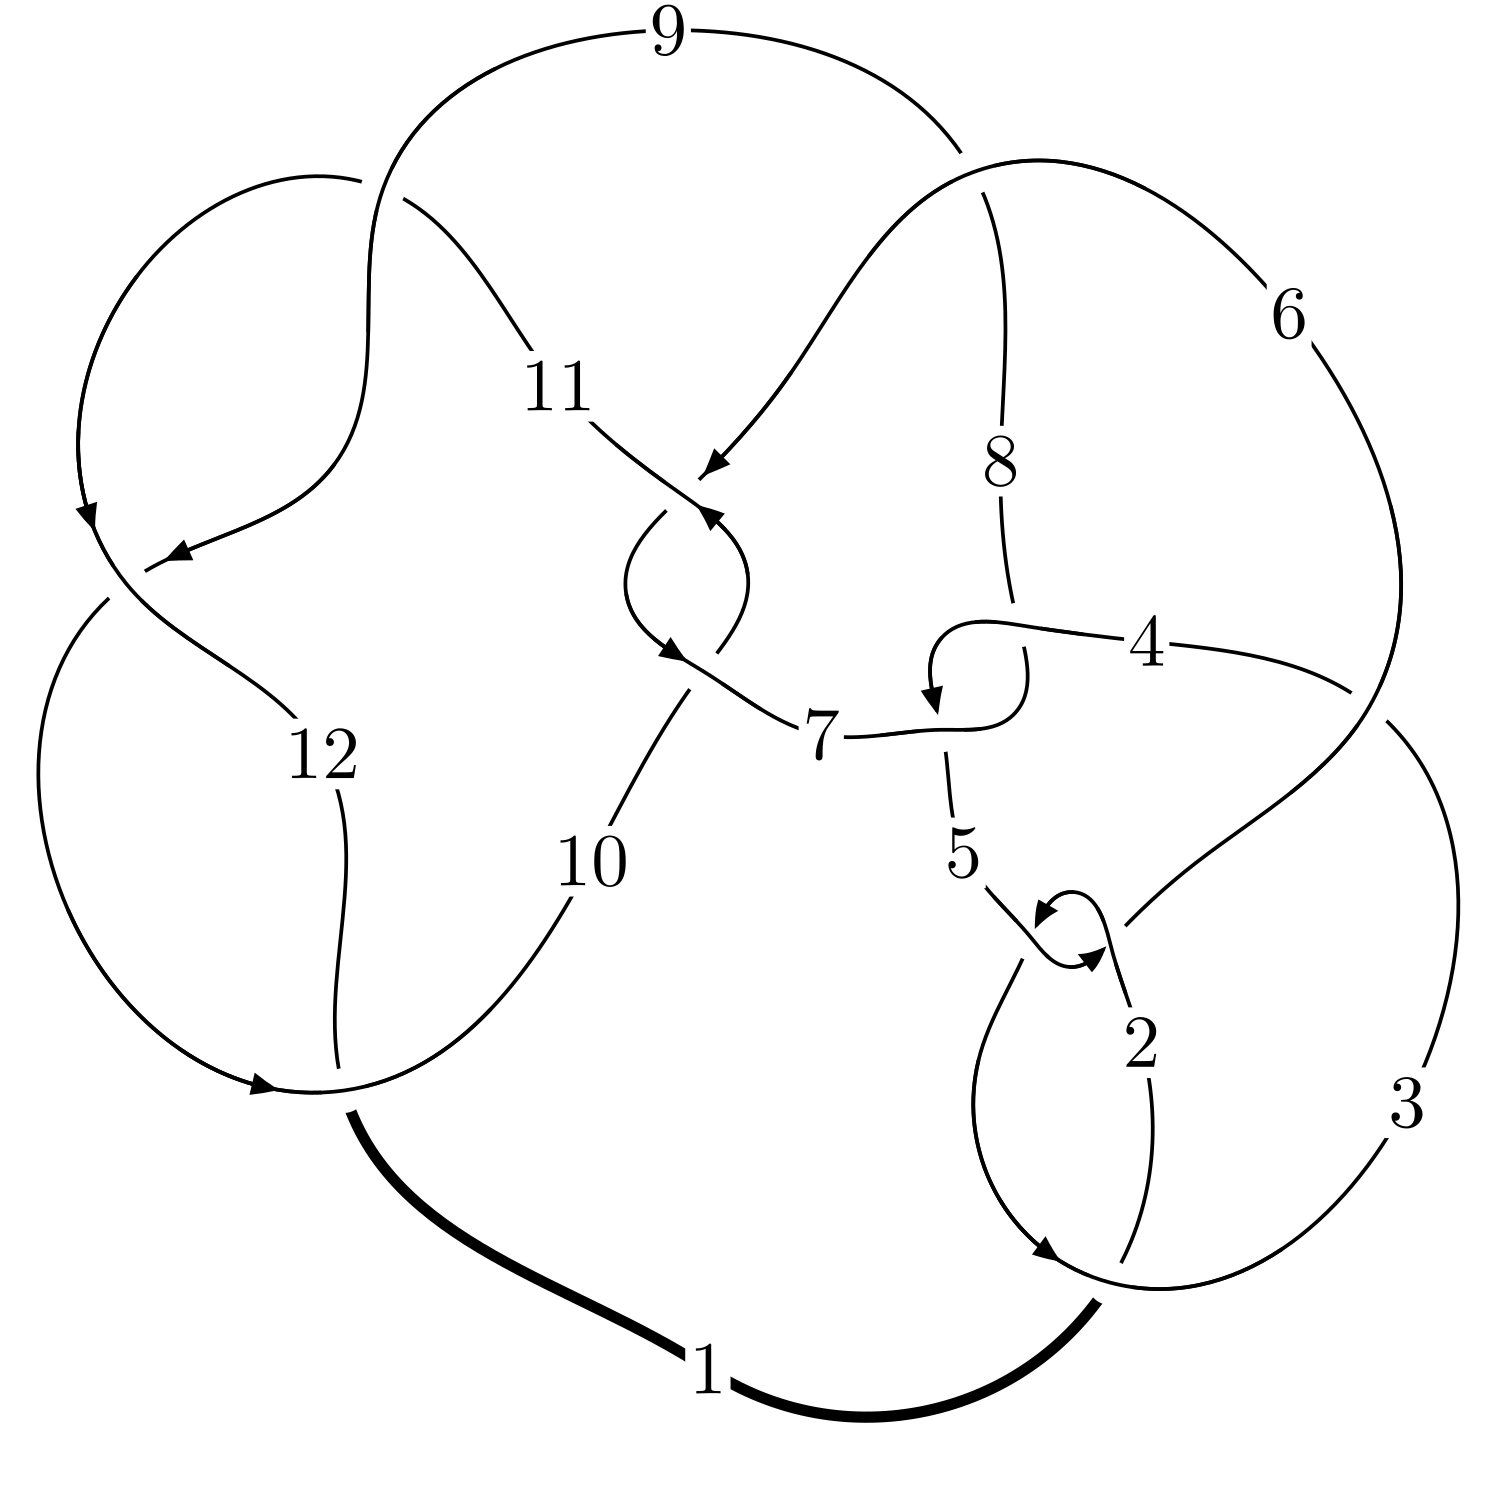
\includegraphics[width=112pt]{../../../GIT/diagram.site/Diagrams/png/2098_12n_0009.png}\\
\ \ \ A knot diagram\footnotemark}&
\allowdisplaybreaks
\textbf{Linearized knot diagam} \\
\cline{2-2}
 &
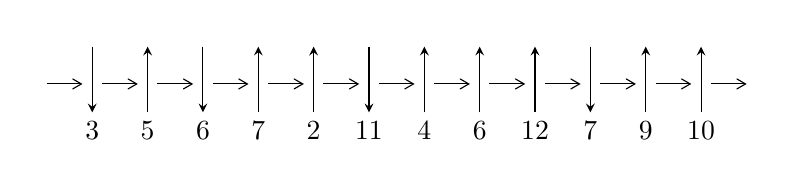
\begin{tikzpicture}[x=20pt, y=17pt]
	% nodes
	\node (C0) at (0, 0) {};
	\node (C1) at (1, 0) {};
	\node (C1U) at (1, +1) {};
	\node (C1D) at (1, -1) {3};

	\node (C2) at (2, 0) {};
	\node (C2U) at (2, +1) {};
	\node (C2D) at (2, -1) {5};

	\node (C3) at (3, 0) {};
	\node (C3U) at (3, +1) {};
	\node (C3D) at (3, -1) {6};

	\node (C4) at (4, 0) {};
	\node (C4U) at (4, +1) {};
	\node (C4D) at (4, -1) {7};

	\node (C5) at (5, 0) {};
	\node (C5U) at (5, +1) {};
	\node (C5D) at (5, -1) {2};

	\node (C6) at (6, 0) {};
	\node (C6U) at (6, +1) {};
	\node (C6D) at (6, -1) {11};

	\node (C7) at (7, 0) {};
	\node (C7U) at (7, +1) {};
	\node (C7D) at (7, -1) {4};

	\node (C8) at (8, 0) {};
	\node (C8U) at (8, +1) {};
	\node (C8D) at (8, -1) {6};

	\node (C9) at (9, 0) {};
	\node (C9U) at (9, +1) {};
	\node (C9D) at (9, -1) {12};

	\node (C10) at (10, 0) {};
	\node (C10U) at (10, +1) {};
	\node (C10D) at (10, -1) {7};

	\node (C11) at (11, 0) {};
	\node (C11U) at (11, +1) {};
	\node (C11D) at (11, -1) {9};

	\node (C12) at (12, 0) {};
	\node (C12U) at (12, +1) {};
	\node (C12D) at (12, -1) {10};
	\node (C13) at (13, 0) {};

	% arrows
	\draw[->,>={angle 60}]
	(C0) edge (C1) (C1) edge (C2) (C2) edge (C3) (C3) edge (C4) (C4) edge (C5) (C5) edge (C6) (C6) edge (C7) (C7) edge (C8) (C8) edge (C9) (C9) edge (C10) (C10) edge (C11) (C11) edge (C12) (C12) edge (C13) ;	\draw[->,>=stealth]
	(C1U) edge (C1D) (C2D) edge (C2U) (C3U) edge (C3D) (C4D) edge (C4U) (C5D) edge (C5U) (C6U) edge (C6D) (C7D) edge (C7U) (C8D) edge (C8U) (C9D) edge (C9U) (C10U) edge (C10D) (C11D) edge (C11U) (C12D) edge (C12U) ;
	\end{tikzpicture} \\
\hhline{~~} \\& 
\textbf{Solving Sequence} \\ \cline{2-2} 
 &
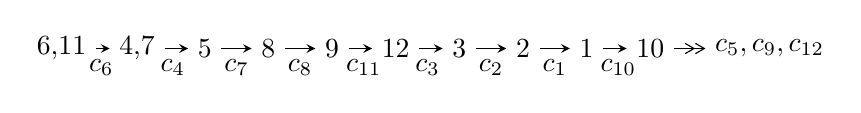
\begin{tikzpicture}[x=23pt, y=7pt]
	% node
	\node (A0) at (-1/8, 0) {6,11};
	\node (A1) at (17/16, 0) {4,7};
	\node (A2) at (17/8, 0) {5};
	\node (A3) at (25/8, 0) {8};
	\node (A4) at (33/8, 0) {9};
	\node (A5) at (41/8, 0) {12};
	\node (A6) at (49/8, 0) {3};
	\node (A7) at (57/8, 0) {2};
	\node (A8) at (65/8, 0) {1};
	\node (A9) at (73/8, 0) {10};
	\node (C1) at (1/2, -1) {$c_{6}$};
	\node (C2) at (13/8, -1) {$c_{4}$};
	\node (C3) at (21/8, -1) {$c_{7}$};
	\node (C4) at (29/8, -1) {$c_{8}$};
	\node (C5) at (37/8, -1) {$c_{11}$};
	\node (C6) at (45/8, -1) {$c_{3}$};
	\node (C7) at (53/8, -1) {$c_{2}$};
	\node (C8) at (61/8, -1) {$c_{1}$};
	\node (C9) at (69/8, -1) {$c_{10}$};
	\node (A10) at (11, 0) {$c_{5},c_{9},c_{12}$};

	% edge
	\draw[->,>=stealth]	
	(A0) edge (A1) (A1) edge (A2) (A2) edge (A3) (A3) edge (A4) (A4) edge (A5) (A5) edge (A6) (A6) edge (A7) (A7) edge (A8) (A8) edge (A9) ;
	\draw[->>,>={angle 60}]	
	(A9) edge (A10);
\end{tikzpicture} \\ 

\end{tabular} \\

\footnotetext{
The image of knot diagram is generated by the software ``\textbf{Draw programme}" developed by Andrew Bartholomew(\url{http://www.layer8.co.uk/maths/draw/index.htm\#Running-draw}), where we modified some parts for our purpose(\url{https://github.com/CATsTAILs/LinksPainter}).
}\phantom \\ \newline 
\centering \textbf{Ideals for irreducible components\footnotemark of $X_{\text{par}}$} 
 
\begin{align*}
I^u_{1}&=\langle 
2.21642\times10^{44} u^{44}-9.65342\times10^{44} u^{43}+\cdots+5.80500\times10^{44} b+4.56035\times10^{43},\\
\phantom{I^u_{1}}&\phantom{= \langle  }-9.69683\times10^{44} u^{44}+2.59441\times10^{45} u^{43}+\cdots+5.80500\times10^{44} a-1.42142\times10^{45},\;u^{45}-3 u^{44}+\cdots-2 u+1\rangle \\
I^u_{2}&=\langle 
- u^2 a+b,\;u^4 a+u^4+u^2 a+u^3+a^2- a u+3 u^2+u+2,\;u^5+u^4+2 u^3+u^2+u+1\rangle \\
\\
\end{align*}
\raggedright * 2 irreducible components of $\dim_{\mathbb{C}}=0$, with total 55 representations.\\
\footnotetext{All coefficients of polynomials are rational numbers. But the coefficients are sometimes approximated in decimal forms when there is not enough margin.}
\newpage
\renewcommand{\arraystretch}{1}
\centering \section*{I. $I^u_{1}= \langle 2.22\times10^{44} u^{44}-9.65\times10^{44} u^{43}+\cdots+5.80\times10^{44} b+4.56\times10^{43},\;-9.70\times10^{44} u^{44}+2.59\times10^{45} u^{43}+\cdots+5.80\times10^{44} a-1.42\times10^{45},\;u^{45}-3 u^{44}+\cdots-2 u+1 \rangle$}
\flushleft \textbf{(i) Arc colorings}\\
\begin{tabular}{m{7pt} m{180pt} m{7pt} m{180pt} }
\flushright $a_{6}=$&$\begin{pmatrix}1\\0\end{pmatrix}$ \\
\flushright $a_{11}=$&$\begin{pmatrix}0\\u\end{pmatrix}$ \\
\flushright $a_{4}=$&$\begin{pmatrix}1.67043 u^{44}-4.46927 u^{43}+\cdots+1.43251 u+2.44861\\-0.381812 u^{44}+1.66295 u^{43}+\cdots-2.28564 u-0.0785591\end{pmatrix}$ \\
\flushright $a_{7}=$&$\begin{pmatrix}1\\u^2\end{pmatrix}$ \\
\flushright $a_{5}=$&$\begin{pmatrix}1.52725 u^{44}-3.73078 u^{43}+\cdots-0.266722 u+2.91206\\-0.353492 u^{44}+1.38147 u^{43}+\cdots-1.52456 u-0.387507\end{pmatrix}$ \\
\flushright $a_{8}=$&$\begin{pmatrix}0.180463 u^{44}-0.229067 u^{43}+\cdots-0.106601 u-0.509733\\0.932433 u^{44}-3.31426 u^{43}+\cdots+3.71638 u-1.49789\end{pmatrix}$ \\
\flushright $a_{9}=$&$\begin{pmatrix}1.11290 u^{44}-3.54332 u^{43}+\cdots+3.60978 u-2.00762\\0.932433 u^{44}-3.31426 u^{43}+\cdots+3.71638 u-1.49789\end{pmatrix}$ \\
\flushright $a_{12}=$&$\begin{pmatrix}0.107422 u^{44}-0.715021 u^{43}+\cdots+1.62877 u+0.305097\\0.795848 u^{44}-2.98218 u^{43}+\cdots+4.34562 u-1.30977\end{pmatrix}$ \\
\flushright $a_{3}=$&$\begin{pmatrix}1.28862 u^{44}-2.80632 u^{43}+\cdots-0.853129 u+2.37005\\-0.381812 u^{44}+1.66295 u^{43}+\cdots-2.28564 u-0.0785591\end{pmatrix}$ \\
\flushright $a_{2}=$&$\begin{pmatrix}0.248367 u^{44}-0.966971 u^{43}+\cdots+5.08102 u+1.34780\\-0.418841 u^{44}+1.39898 u^{43}+\cdots-1.39587 u+0.364330\end{pmatrix}$ \\
\flushright $a_{1}=$&$\begin{pmatrix}0.180463 u^{44}-0.229067 u^{43}+\cdots-0.106601 u-0.509733\\-0.611791 u^{44}+2.34940 u^{43}+\cdots-3.27220 u+1.18556\end{pmatrix}$ \\
\flushright $a_{10}=$&$\begin{pmatrix}u\\u^3+u\end{pmatrix}$\\&\end{tabular}
\flushleft \textbf{(ii) Obstruction class $= -1$}\\~\\
\flushleft \textbf{(iii) Cusp Shapes $= 6.45073 u^{44}-19.7307 u^{43}+\cdots+14.2789 u-6.88518$}\\~\\
\newpage\renewcommand{\arraystretch}{1}
\flushleft \textbf{(iv) u-Polynomials at the component}\newline \\
\begin{tabular}{m{50pt}|m{274pt}}
Crossings & \hspace{64pt}u-Polynomials at each crossing \\
\hline $$\begin{aligned}c_{1}\end{aligned}$$&$\begin{aligned}
&u^{45}+28 u^{44}+\cdots+13 u-1
\end{aligned}$\\
\hline $$\begin{aligned}c_{2},c_{5}\end{aligned}$$&$\begin{aligned}
&u^{45}+6 u^{44}+\cdots+u-1
\end{aligned}$\\
\hline $$\begin{aligned}c_{3}\end{aligned}$$&$\begin{aligned}
&u^{45}-6 u^{44}+\cdots+11 u-1
\end{aligned}$\\
\hline $$\begin{aligned}c_{4},c_{7}\end{aligned}$$&$\begin{aligned}
&u^{45}+3 u^{44}+\cdots-2048 u+1024
\end{aligned}$\\
\hline $$\begin{aligned}c_{6},c_{10}\end{aligned}$$&$\begin{aligned}
&u^{45}+3 u^{44}+\cdots-2 u-1
\end{aligned}$\\
\hline $$\begin{aligned}c_{8}\end{aligned}$$&$\begin{aligned}
&u^{45}+9 u^{44}+\cdots-305892 u+52489
\end{aligned}$\\
\hline $$\begin{aligned}c_{9},c_{11},c_{12}\end{aligned}$$&$\begin{aligned}
&u^{45}+3 u^{44}+\cdots+8 u-1
\end{aligned}$\\
\hline
\end{tabular}\\~\\
\newpage\renewcommand{\arraystretch}{1}
\flushleft \textbf{(v) Riley Polynomials at the component}\newline \\
\begin{tabular}{m{50pt}|m{274pt}}
Crossings & \hspace{64pt}Riley Polynomials at each crossing \\
\hline $$\begin{aligned}c_{1}\end{aligned}$$&$\begin{aligned}
&y^{45}-16 y^{44}+\cdots+2813 y-1
\end{aligned}$\\
\hline $$\begin{aligned}c_{2},c_{5}\end{aligned}$$&$\begin{aligned}
&y^{45}+28 y^{44}+\cdots+13 y-1
\end{aligned}$\\
\hline $$\begin{aligned}c_{3}\end{aligned}$$&$\begin{aligned}
&y^{45}-60 y^{44}+\cdots+13 y-1
\end{aligned}$\\
\hline $$\begin{aligned}c_{4},c_{7}\end{aligned}$$&$\begin{aligned}
&y^{45}+55 y^{44}+\cdots-12582912 y-1048576
\end{aligned}$\\
\hline $$\begin{aligned}c_{6},c_{10}\end{aligned}$$&$\begin{aligned}
&y^{45}+9 y^{44}+\cdots-8 y-1
\end{aligned}$\\
\hline $$\begin{aligned}c_{8}\end{aligned}$$&$\begin{aligned}
&y^{45}+37 y^{44}+\cdots-75656299984 y-2755095121
\end{aligned}$\\
\hline $$\begin{aligned}c_{9},c_{11},c_{12}\end{aligned}$$&$\begin{aligned}
&y^{45}-35 y^{44}+\cdots-8 y-1
\end{aligned}$\\
\hline
\end{tabular}\\~\\
\newpage\flushleft \textbf{(vi) Complex Volumes and Cusp Shapes}
$$\begin{array}{c|c|c}  
\text{Solutions to }I^u_{1}& \I (\text{vol} + \sqrt{-1}CS) & \text{Cusp shape}\\
 \hline 
\begin{aligned}
u &= -0.996119 + 0.282709 I \\
a &= \phantom{-}0.110387 + 0.980594 I \\
b &= \phantom{-}0.080579 + 0.175761 I\end{aligned}
 & \phantom{-}1.42637 - 0.55806 I & \phantom{-}2.83426 - 0.60220 I \\ \hline\begin{aligned}
u &= -0.996119 - 0.282709 I \\
a &= \phantom{-}0.110387 - 0.980594 I \\
b &= \phantom{-}0.080579 - 0.175761 I\end{aligned}
 & \phantom{-}1.42637 + 0.55806 I & \phantom{-}2.83426 + 0.60220 I \\ \hline\begin{aligned}
u &= \phantom{-}0.783242 + 0.506620 I \\
a &= -0.030126 - 0.893560 I \\
b &= -0.396180 + 0.324015 I\end{aligned}
 & -3.24493 - 1.98845 I & -2.05742 + 2.49039 I \\ \hline\begin{aligned}
u &= \phantom{-}0.783242 - 0.506620 I \\
a &= -0.030126 + 0.893560 I \\
b &= -0.396180 - 0.324015 I\end{aligned}
 & -3.24493 + 1.98845 I & -2.05742 - 2.49039 I \\ \hline\begin{aligned}
u &= -0.647911 + 0.616131 I \\
a &= \phantom{-}0.277858 + 0.505783 I \\
b &= -1.283800 - 0.505811 I\end{aligned}
 & -0.49292 + 5.46151 I & \phantom{-}3.53146 - 8.21286 I \\ \hline\begin{aligned}
u &= -0.647911 - 0.616131 I \\
a &= \phantom{-}0.277858 - 0.505783 I \\
b &= -1.283800 + 0.505811 I\end{aligned}
 & -0.49292 - 5.46151 I & \phantom{-}3.53146 + 8.21286 I \\ \hline\begin{aligned}
u &= \phantom{-}0.415458 + 1.074940 I \\
a &= -0.242176 + 0.556359 I \\
b &= \phantom{-}0.272242 + 0.056149 I\end{aligned}
 & -1.16555 - 2.65109 I & \phantom{-}0.66724 + 3.06904 I \\ \hline\begin{aligned}
u &= \phantom{-}0.415458 - 1.074940 I \\
a &= -0.242176 - 0.556359 I \\
b &= \phantom{-}0.272242 - 0.056149 I\end{aligned}
 & -1.16555 + 2.65109 I & \phantom{-}0.66724 - 3.06904 I \\ \hline\begin{aligned}
u &= -0.300364 + 0.770681 I \\
a &= \phantom{-}0.78986 - 1.26679 I \\
b &= -0.252806 - 0.197943 I\end{aligned}
 & \phantom{-}0.37099 - 1.66366 I & \phantom{-}5.28694 + 1.76198 I \\ \hline\begin{aligned}
u &= -0.300364 - 0.770681 I \\
a &= \phantom{-}0.78986 + 1.26679 I \\
b &= -0.252806 + 0.197943 I\end{aligned}
 & \phantom{-}0.37099 + 1.66366 I & \phantom{-}5.28694 - 1.76198 I\\
 \hline 
 \end{array}$$\newpage$$\begin{array}{c|c|c}  
\text{Solutions to }I^u_{1}& \I (\text{vol} + \sqrt{-1}CS) & \text{Cusp shape}\\
 \hline 
\begin{aligned}
u &= -0.349037 + 1.204480 I \\
a &= \phantom{-}0.230921 - 0.225780 I \\
b &= -0.048432 + 0.642308 I\end{aligned}
 & \phantom{-}6.11434 + 3.25836 I & \phantom{-}9.12554 - 6.20048 I \\ \hline\begin{aligned}
u &= -0.349037 - 1.204480 I \\
a &= \phantom{-}0.230921 + 0.225780 I \\
b &= -0.048432 - 0.642308 I\end{aligned}
 & \phantom{-}6.11434 - 3.25836 I & \phantom{-}9.12554 + 6.20048 I \\ \hline\begin{aligned}
u &= \phantom{-}0.224318 + 0.711056 I \\
a &= \phantom{-}0.683426 + 0.176982 I \\
b &= -0.044045 - 0.249882 I\end{aligned}
 & \phantom{-}0.376942 - 1.142080 I & \phantom{-}4.49943 + 6.11117 I \\ \hline\begin{aligned}
u &= \phantom{-}0.224318 - 0.711056 I \\
a &= \phantom{-}0.683426 - 0.176982 I \\
b &= -0.044045 + 0.249882 I\end{aligned}
 & \phantom{-}0.376942 + 1.142080 I & \phantom{-}4.49943 - 6.11117 I \\ \hline\begin{aligned}
u &= -0.084183 + 0.723735 I \\
a &= -0.081939 - 0.906872 I \\
b &= \phantom{-}1.06476 + 1.42506 I\end{aligned}
 & \phantom{-}4.88394 + 1.66123 I & \phantom{-}14.9262 - 3.5385 I \\ \hline\begin{aligned}
u &= -0.084183 - 0.723735 I \\
a &= -0.081939 + 0.906872 I \\
b &= \phantom{-}1.06476 - 1.42506 I\end{aligned}
 & \phantom{-}4.88394 - 1.66123 I & \phantom{-}14.9262 + 3.5385 I \\ \hline\begin{aligned}
u &= \phantom{-}0.315867 + 0.654924 I \\
a &= \phantom{-}0.133646 + 1.369790 I \\
b &= -1.28532 - 1.81254 I\end{aligned}
 & \phantom{-}3.26588 - 4.39540 I & \phantom{-}10.11446 + 8.40755 I \\ \hline\begin{aligned}
u &= \phantom{-}0.315867 - 0.654924 I \\
a &= \phantom{-}0.133646 - 1.369790 I \\
b &= -1.28532 + 1.81254 I\end{aligned}
 & \phantom{-}3.26588 + 4.39540 I & \phantom{-}10.11446 - 8.40755 I \\ \hline\begin{aligned}
u &= \phantom{-}0.928999 + 0.912938 I \\
a &= \phantom{-}1.01128 + 1.05587 I \\
b &= -1.83892 + 0.11929 I\end{aligned}
 & -3.43407 + 1.56417 I & \phantom{-0.000000 } 0 \\ \hline\begin{aligned}
u &= \phantom{-}0.928999 - 0.912938 I \\
a &= \phantom{-}1.01128 - 1.05587 I \\
b &= -1.83892 - 0.11929 I\end{aligned}
 & -3.43407 - 1.56417 I & \phantom{-0.000000 } 0\\
 \hline 
 \end{array}$$\newpage$$\begin{array}{c|c|c}  
\text{Solutions to }I^u_{1}& \I (\text{vol} + \sqrt{-1}CS) & \text{Cusp shape}\\
 \hline 
\begin{aligned}
u &= \phantom{-}1.004980 + 0.829128 I \\
a &= -0.550201 - 1.282520 I \\
b &= \phantom{-}1.72749 + 0.74464 I\end{aligned}
 & -8.38531 - 3.39936 I & \phantom{-0.000000 } 0 \\ \hline\begin{aligned}
u &= \phantom{-}1.004980 - 0.829128 I \\
a &= -0.550201 + 1.282520 I \\
b &= \phantom{-}1.72749 - 0.74464 I\end{aligned}
 & -8.38531 + 3.39936 I & \phantom{-0.000000 } 0 \\ \hline\begin{aligned}
u &= -0.918792 + 0.952300 I \\
a &= \phantom{-}0.87791 - 1.25175 I \\
b &= -2.04722 + 0.30573 I\end{aligned}
 & -7.36187 + 3.39187 I & \phantom{-0.000000 } 0 \\ \hline\begin{aligned}
u &= -0.918792 - 0.952300 I \\
a &= \phantom{-}0.87791 + 1.25175 I \\
b &= -2.04722 - 0.30573 I\end{aligned}
 & -7.36187 - 3.39187 I & \phantom{-0.000000 } 0 \\ \hline\begin{aligned}
u &= \phantom{-}0.908778 + 0.983223 I \\
a &= \phantom{-}0.68380 + 1.36694 I \\
b &= -2.05663 - 0.74421 I\end{aligned}
 & -3.22324 - 8.34361 I & \phantom{-0.000000 } 0 \\ \hline\begin{aligned}
u &= \phantom{-}0.908778 - 0.983223 I \\
a &= \phantom{-}0.68380 - 1.36694 I \\
b &= -2.05663 + 0.74421 I\end{aligned}
 & -3.22324 + 8.34361 I & \phantom{-0.000000 } 0 \\ \hline\begin{aligned}
u &= -1.045050 + 0.865904 I \\
a &= -0.726480 + 1.134250 I \\
b &= \phantom{-}1.94070 - 0.29376 I\end{aligned}
 & -11.88600 - 1.79976 I & \phantom{-0.000000 } 0 \\ \hline\begin{aligned}
u &= -1.045050 - 0.865904 I \\
a &= -0.726480 - 1.134250 I \\
b &= \phantom{-}1.94070 + 0.29376 I\end{aligned}
 & -11.88600 + 1.79976 I & \phantom{-0.000000 } 0 \\ \hline\begin{aligned}
u &= \phantom{-}0.871713 + 1.077210 I \\
a &= -1.17410 - 0.85705 I \\
b &= \phantom{-}1.83482 - 0.04447 I\end{aligned}
 & -7.57148 - 3.49814 I & \phantom{-0.000000 } 0 \\ \hline\begin{aligned}
u &= \phantom{-}0.871713 - 1.077210 I \\
a &= -1.17410 + 0.85705 I \\
b &= \phantom{-}1.83482 + 0.04447 I\end{aligned}
 & -7.57148 + 3.49814 I & \phantom{-0.000000 } 0\\
 \hline 
 \end{array}$$\newpage$$\begin{array}{c|c|c}  
\text{Solutions to }I^u_{1}& \I (\text{vol} + \sqrt{-1}CS) & \text{Cusp shape}\\
 \hline 
\begin{aligned}
u &= \phantom{-}1.086870 + 0.893598 I \\
a &= -0.799128 - 0.940104 I \\
b &= \phantom{-}1.90700 - 0.12468 I\end{aligned}
 & -7.31081 + 6.80058 I & \phantom{-0.000000 } 0 \\ \hline\begin{aligned}
u &= \phantom{-}1.086870 - 0.893598 I \\
a &= -0.799128 + 0.940104 I \\
b &= \phantom{-}1.90700 + 0.12468 I\end{aligned}
 & -7.31081 - 6.80058 I & \phantom{-0.000000 } 0 \\ \hline\begin{aligned}
u &= -0.510690 + 1.315230 I \\
a &= -0.303054 - 0.084448 I \\
b &= \phantom{-}0.565338 - 0.295471 I\end{aligned}
 & \phantom{-}4.91496 + 6.28302 I & \phantom{-0.000000 } 0 \\ \hline\begin{aligned}
u &= -0.510690 - 1.315230 I \\
a &= -0.303054 + 0.084448 I \\
b &= \phantom{-}0.565338 + 0.295471 I\end{aligned}
 & \phantom{-}4.91496 - 6.28302 I & \phantom{-0.000000 } 0 \\ \hline\begin{aligned}
u &= -0.915870 + 1.077500 I \\
a &= -1.01938 + 1.15677 I \\
b &= \phantom{-}2.08407 - 0.22155 I\end{aligned}
 & -11.1799 + 8.9578 I & \phantom{-0.000000 } 0 \\ \hline\begin{aligned}
u &= -0.915870 - 1.077500 I \\
a &= -1.01938 - 1.15677 I \\
b &= \phantom{-}2.08407 + 0.22155 I\end{aligned}
 & -11.1799 - 8.9578 I & \phantom{-0.000000 } 0 \\ \hline\begin{aligned}
u &= -0.039688 + 0.578919 I \\
a &= \phantom{-}1.94846 + 0.78209 I \\
b &= -0.187471 - 0.759973 I\end{aligned}
 & \phantom{-}0.66871 - 1.39964 I & \phantom{-}7.21689 + 5.45878 I \\ \hline\begin{aligned}
u &= -0.039688 - 0.578919 I \\
a &= \phantom{-}1.94846 - 0.78209 I \\
b &= -0.187471 + 0.759973 I\end{aligned}
 & \phantom{-}0.66871 + 1.39964 I & \phantom{-}7.21689 - 5.45878 I \\ \hline\begin{aligned}
u &= -0.571271\phantom{ +0.000000I} \\
a &= \phantom{-}1.59952\phantom{ +0.000000I} \\
b &= \phantom{-}0.143336\phantom{ +0.000000I}\end{aligned}
 & \phantom{-}2.17682\phantom{ +0.000000I} & \phantom{-}3.08930\phantom{ +0.000000I} \\ \hline\begin{aligned}
u &= \phantom{-}0.94832 + 1.08708 I \\
a &= -0.78152 - 1.29730 I \\
b &= \phantom{-}2.14143 + 0.52643 I\end{aligned}
 & -6.6450 - 14.1896 I & \phantom{-0.000000 } 0\\
 \hline 
 \end{array}$$\newpage$$\begin{array}{c|c|c}  
\text{Solutions to }I^u_{1}& \I (\text{vol} + \sqrt{-1}CS) & \text{Cusp shape}\\
 \hline 
\begin{aligned}
u &= \phantom{-}0.94832 - 1.08708 I \\
a &= -0.78152 + 1.29730 I \\
b &= \phantom{-}2.14143 - 0.52643 I\end{aligned}
 & -6.6450 + 14.1896 I & \phantom{-0.000000 } 0 \\ \hline\begin{aligned}
u &= -0.323389 + 0.438179 I \\
a &= -1.32309 - 1.43900 I \\
b &= -0.774207 + 0.940763 I\end{aligned}
 & -0.07007 + 2.75890 I & \phantom{-}1.271024 - 0.509737 I \\ \hline\begin{aligned}
u &= -0.323389 - 0.438179 I \\
a &= -1.32309 + 1.43900 I \\
b &= -0.774207 - 0.940763 I\end{aligned}
 & -0.07007 - 2.75890 I & \phantom{-}1.271024 + 0.509737 I \\ \hline\begin{aligned}
u &= \phantom{-}0.428186 + 0.132966 I \\
a &= \phantom{-}1.98389 + 7.20476 I \\
b &= -0.475066 + 0.996976 I\end{aligned}
 & \phantom{-}1.97991 + 2.18754 I & -20.6628 + 4.9777 I \\ \hline\begin{aligned}
u &= \phantom{-}0.428186 - 0.132966 I \\
a &= \phantom{-}1.98389 - 7.20476 I \\
b &= -0.475066 - 0.996976 I\end{aligned}
 & \phantom{-}1.97991 - 2.18754 I & -20.6628 - 4.9777 I\\
 \hline 
 \end{array}$$\newpage\newpage\renewcommand{\arraystretch}{1}
\centering \section*{II. $I^u_{2}= \langle - u^2 a+b,\;u^4 a+u^4+u^2 a+u^3+a^2- a u+3 u^2+u+2,\;u^5+u^4+2 u^3+u^2+u+1 \rangle$}
\flushleft \textbf{(i) Arc colorings}\\
\begin{tabular}{m{7pt} m{180pt} m{7pt} m{180pt} }
\flushright $a_{6}=$&$\begin{pmatrix}1\\0\end{pmatrix}$ \\
\flushright $a_{11}=$&$\begin{pmatrix}0\\u\end{pmatrix}$ \\
\flushright $a_{4}=$&$\begin{pmatrix}a\\u^2 a\end{pmatrix}$ \\
\flushright $a_{7}=$&$\begin{pmatrix}1\\u^2\end{pmatrix}$ \\
\flushright $a_{5}=$&$\begin{pmatrix}a\\u^2 a\end{pmatrix}$ \\
\flushright $a_{8}=$&$\begin{pmatrix}1\\u^2\end{pmatrix}$ \\
\flushright $a_{9}=$&$\begin{pmatrix}u^2+1\\u^2\end{pmatrix}$ \\
\flushright $a_{12}=$&$\begin{pmatrix}- u^4- u^2-1\\- u^4- u^3- u^2-1\end{pmatrix}$ \\
\flushright $a_{3}=$&$\begin{pmatrix}u^2 a+a\\u^2 a\end{pmatrix}$ \\
\flushright $a_{2}=$&$\begin{pmatrix}u^4+u^2 a+u^2+a- u\\u^2 a+1\end{pmatrix}$ \\
\flushright $a_{1}=$&$\begin{pmatrix}-1\\0\end{pmatrix}$ \\
\flushright $a_{10}=$&$\begin{pmatrix}u\\u^3+u\end{pmatrix}$\\&\end{tabular}
\flushleft \textbf{(ii) Obstruction class $= 1$}\\~\\
\flushleft \textbf{(iii) Cusp Shapes $= 2 u^4 a- u^3 a+u^4-3 u^2 a+5 u^3- a u+7 u^2- a+5 u+8$}\\~\\
\newpage\renewcommand{\arraystretch}{1}
\flushleft \textbf{(iv) u-Polynomials at the component}\newline \\
\begin{tabular}{m{50pt}|m{274pt}}
Crossings & \hspace{64pt}u-Polynomials at each crossing \\
\hline $$\begin{aligned}c_{1},c_{3},c_{5}\end{aligned}$$&$\begin{aligned}
&(u^2- u+1)^5
\end{aligned}$\\
\hline $$\begin{aligned}c_{2}\end{aligned}$$&$\begin{aligned}
&(u^2+u+1)^5
\end{aligned}$\\
\hline $$\begin{aligned}c_{4},c_{7}\end{aligned}$$&$\begin{aligned}
&u^{10}
\end{aligned}$\\
\hline $$\begin{aligned}c_{6}\end{aligned}$$&$\begin{aligned}
&(u^5+u^4+2 u^3+u^2+u+1)^2
\end{aligned}$\\
\hline $$\begin{aligned}c_{8}\end{aligned}$$&$\begin{aligned}
&(u^5-3 u^4+4 u^3- u^2- u+1)^2
\end{aligned}$\\
\hline $$\begin{aligned}c_{9}\end{aligned}$$&$\begin{aligned}
&(u^5- u^4-2 u^3+u^2+u+1)^2
\end{aligned}$\\
\hline $$\begin{aligned}c_{10}\end{aligned}$$&$\begin{aligned}
&(u^5- u^4+2 u^3- u^2+u-1)^2
\end{aligned}$\\
\hline $$\begin{aligned}c_{11},c_{12}\end{aligned}$$&$\begin{aligned}
&(u^5+u^4-2 u^3- u^2+u-1)^2
\end{aligned}$\\
\hline
\end{tabular}\\~\\
\newpage\renewcommand{\arraystretch}{1}
\flushleft \textbf{(v) Riley Polynomials at the component}\newline \\
\begin{tabular}{m{50pt}|m{274pt}}
Crossings & \hspace{64pt}Riley Polynomials at each crossing \\
\hline $$\begin{aligned}c_{1},c_{2},c_{3}\\c_{5}\end{aligned}$$&$\begin{aligned}
&(y^2+y+1)^5
\end{aligned}$\\
\hline $$\begin{aligned}c_{4},c_{7}\end{aligned}$$&$\begin{aligned}
&y^{10}
\end{aligned}$\\
\hline $$\begin{aligned}c_{6},c_{10}\end{aligned}$$&$\begin{aligned}
&(y^5+3 y^4+4 y^3+y^2- y-1)^2
\end{aligned}$\\
\hline $$\begin{aligned}c_{8}\end{aligned}$$&$\begin{aligned}
&(y^5- y^4+8 y^3-3 y^2+3 y-1)^2
\end{aligned}$\\
\hline $$\begin{aligned}c_{9},c_{11},c_{12}\end{aligned}$$&$\begin{aligned}
&(y^5-5 y^4+8 y^3-3 y^2- y-1)^2
\end{aligned}$\\
\hline
\end{tabular}\\~\\
\newpage\flushleft \textbf{(vi) Complex Volumes and Cusp Shapes}
$$\begin{array}{c|c|c}  
\text{Solutions to }I^u_{2}& \I (\text{vol} + \sqrt{-1}CS) & \text{Cusp shape}\\
 \hline 
\begin{aligned}
u &= \phantom{-}0.339110 + 0.822375 I \\
a &= \phantom{-}1.219640 - 0.330957 I \\
b &= -0.500000 + 0.866025 I\end{aligned}
 & \phantom{-}0.329100 + 0.499304 I & \phantom{-}2.59686 + 1.45733 I \\ \hline\begin{aligned}
u &= \phantom{-}0.339110 + 0.822375 I \\
a &= -0.323203 + 1.221720 I \\
b &= -0.500000 - 0.866025 I\end{aligned}
 & \phantom{-}0.32910 - 3.56046 I & \phantom{-}6.44749 + 8.37485 I \\ \hline\begin{aligned}
u &= \phantom{-}0.339110 - 0.822375 I \\
a &= \phantom{-}1.219640 + 0.330957 I \\
b &= -0.500000 - 0.866025 I\end{aligned}
 & \phantom{-}0.329100 - 0.499304 I & \phantom{-}2.59686 - 1.45733 I \\ \hline\begin{aligned}
u &= \phantom{-}0.339110 - 0.822375 I \\
a &= -0.323203 - 1.221720 I \\
b &= -0.500000 + 0.866025 I\end{aligned}
 & \phantom{-}0.32910 + 3.56046 I & \phantom{-}6.44749 - 8.37485 I \\ \hline\begin{aligned}
u &= -0.766826\phantom{ +0.000000I} \\
a &= -0.85031 + 1.47278 I \\
b &= -0.500000 + 0.866025 I\end{aligned}
 & \phantom{-}2.40108 + 2.02988 I & \phantom{-}7.10008 - 1.25892 I \\ \hline\begin{aligned}
u &= -0.766826\phantom{ +0.000000I} \\
a &= -0.85031 - 1.47278 I \\
b &= -0.500000 - 0.866025 I\end{aligned}
 & \phantom{-}2.40108 - 2.02988 I & \phantom{-}7.10008 + 1.25892 I \\ \hline\begin{aligned}
u &= -0.455697 + 1.200150 I \\
a &= \phantom{-}0.575710 + 0.191698 I \\
b &= -0.500000 - 0.866025 I\end{aligned}
 & \phantom{-}5.87256 + 2.37095 I & \phantom{-}6.27578 + 1.37298 I \\ \hline\begin{aligned}
u &= -0.455697 + 1.200150 I \\
a &= -0.121840 - 0.594429 I \\
b &= -0.500000 + 0.866025 I\end{aligned}
 & \phantom{-}5.87256 + 6.43072 I & \phantom{-}11.57979 - 6.03904 I \\ \hline\begin{aligned}
u &= -0.455697 - 1.200150 I \\
a &= \phantom{-}0.575710 - 0.191698 I \\
b &= -0.500000 + 0.866025 I\end{aligned}
 & \phantom{-}5.87256 - 2.37095 I & \phantom{-}6.27578 - 1.37298 I \\ \hline\begin{aligned}
u &= -0.455697 - 1.200150 I \\
a &= -0.121840 + 0.594429 I \\
b &= -0.500000 - 0.866025 I\end{aligned}
 & \phantom{-}5.87256 - 6.43072 I & \phantom{-}11.57979 + 6.03904 I\\
 \hline 
 \end{array}$$\newpage
\newpage\renewcommand{\arraystretch}{1}
\centering \section*{ III. u-Polynomials}
\begin{tabular}{m{50pt}|m{274pt}}
Crossings & \hspace{64pt}u-Polynomials at each crossing \\
\hline $$\begin{aligned}c_{1}\end{aligned}$$&$\begin{aligned}
&((u^2- u+1)^5)(u^{45}+28 u^{44}+\cdots+13 u-1)
\end{aligned}$\\
\hline $$\begin{aligned}c_{2}\end{aligned}$$&$\begin{aligned}
&((u^2+u+1)^5)(u^{45}+6 u^{44}+\cdots+u-1)
\end{aligned}$\\
\hline $$\begin{aligned}c_{3}\end{aligned}$$&$\begin{aligned}
&((u^2- u+1)^5)(u^{45}-6 u^{44}+\cdots+11 u-1)
\end{aligned}$\\
\hline $$\begin{aligned}c_{4},c_{7}\end{aligned}$$&$\begin{aligned}
&u^{10}(u^{45}+3 u^{44}+\cdots-2048 u+1024)
\end{aligned}$\\
\hline $$\begin{aligned}c_{5}\end{aligned}$$&$\begin{aligned}
&((u^2- u+1)^5)(u^{45}+6 u^{44}+\cdots+u-1)
\end{aligned}$\\
\hline $$\begin{aligned}c_{6}\end{aligned}$$&$\begin{aligned}
&((u^5+u^4+2 u^3+u^2+u+1)^2)(u^{45}+3 u^{44}+\cdots-2 u-1)
\end{aligned}$\\
\hline $$\begin{aligned}c_{8}\end{aligned}$$&$\begin{aligned}
&((u^5-3 u^4+4 u^3- u^2- u+1)^2)(u^{45}+9 u^{44}+\cdots-305892 u+52489)
\end{aligned}$\\
\hline $$\begin{aligned}c_{9}\end{aligned}$$&$\begin{aligned}
&((u^5- u^4-2 u^3+u^2+u+1)^2)(u^{45}+3 u^{44}+\cdots+8 u-1)
\end{aligned}$\\
\hline $$\begin{aligned}c_{10}\end{aligned}$$&$\begin{aligned}
&((u^5- u^4+2 u^3- u^2+u-1)^2)(u^{45}+3 u^{44}+\cdots-2 u-1)
\end{aligned}$\\
\hline $$\begin{aligned}c_{11},c_{12}\end{aligned}$$&$\begin{aligned}
&((u^5+u^4-2 u^3- u^2+u-1)^2)(u^{45}+3 u^{44}+\cdots+8 u-1)
\end{aligned}$\\
\hline
\end{tabular}\newpage\renewcommand{\arraystretch}{1}
\centering \section*{ IV. Riley Polynomials}
\begin{tabular}{m{50pt}|m{274pt}}
Crossings & \hspace{64pt}Riley Polynomials at each crossing \\
\hline $$\begin{aligned}c_{1}\end{aligned}$$&$\begin{aligned}
&((y^2+y+1)^5)(y^{45}-16 y^{44}+\cdots+2813 y-1)
\end{aligned}$\\
\hline $$\begin{aligned}c_{2},c_{5}\end{aligned}$$&$\begin{aligned}
&((y^2+y+1)^5)(y^{45}+28 y^{44}+\cdots+13 y-1)
\end{aligned}$\\
\hline $$\begin{aligned}c_{3}\end{aligned}$$&$\begin{aligned}
&((y^2+y+1)^5)(y^{45}-60 y^{44}+\cdots+13 y-1)
\end{aligned}$\\
\hline $$\begin{aligned}c_{4},c_{7}\end{aligned}$$&$\begin{aligned}
&y^{10}(y^{45}+55 y^{44}+\cdots-1.25829\times10^{7} y-1048576)
\end{aligned}$\\
\hline $$\begin{aligned}c_{6},c_{10}\end{aligned}$$&$\begin{aligned}
&((y^5+3 y^4+4 y^3+y^2- y-1)^2)(y^{45}+9 y^{44}+\cdots-8 y-1)
\end{aligned}$\\
\hline $$\begin{aligned}c_{8}\end{aligned}$$&$\begin{aligned}
&(y^5- y^4+8 y^3-3 y^2+3 y-1)^2\\
&\cdot(y^{45}+37 y^{44}+\cdots-75656299984 y-2755095121)
\end{aligned}$\\
\hline $$\begin{aligned}c_{9},c_{11},c_{12}\end{aligned}$$&$\begin{aligned}
&((y^5-5 y^4+8 y^3-3 y^2- y-1)^2)(y^{45}-35 y^{44}+\cdots-8 y-1)
\end{aligned}$\\
\hline
\end{tabular}
\vskip 2pc
\end{document}